%%%%%%%%%%%%%%%%%%%%%%%%%%%%%%%%%%%%%%%%%
% Short Sectioned Assignment
% LaTeX Template
% Version 1.0 (5/5/12)
%
% This template has been downloaded from:
% http://www.LaTeXTemplates.com
%
% Original author:
% Frits Wenneker (http://www.howtotex.com)
%
% License:
% CC BY-NC-SA 3.0 (http://creativecommons.org/licenses/by-nc-sa/3.0/)
%
%%%%%%%%%%%%%%%%%%%%%%%%%%%%%%%%%%%%%%%%%

%----------------------------------------------------------------------------------------
%	PACKAGES AND OTHER DOCUMENT CONFIGURATIONS
%----------------------------------------------------------------------------------------

\documentclass[paper=a4, fontsize=11pt]{scrartcl} % A4 paper and 11pt font size

\usepackage[T1]{fontenc} % Use 8-bit encoding that has 256 glyphs
\usepackage{fourier} % Use the Adobe Utopia font for the document - comment this line to return to the LaTeX default
\usepackage[english]{babel} % English language/hyphenation
\usepackage{amsmath,amsfonts,amsthm} % Math packages
\usepackage{listings}
\usepackage{graphicx}
%\graphicspath{ {Desktop/PA3_numerical_analysis/} }

\usepackage{lipsum} % Used for inserting dummy 'Lorem ipsum' text into the template

\usepackage{sectsty} % Allows customizing section commands
\allsectionsfont{\centering \normalfont\scshape} % Make all sections centered, the default font and small caps

\usepackage{fancyhdr} % Custom headers and footers
\pagestyle{fancyplain} % Makes all pages in the document conform to the custom headers and footers
\fancyhead{} % No page header - if you want one, create it in the same way as the footers below
\fancyfoot[L]{} % Empty left footer
\fancyfoot[C]{} % Empty center footer
\fancyfoot[R]{\thepage} % Page numbering for right footer
\renewcommand{\headrulewidth}{0pt} % Remove header underlines
\renewcommand{\footrulewidth}{0pt} % Remove footer underlines
\setlength{\headheight}{13.6pt} % Customize the height of the header

\numberwithin{equation}{section} % Number equations within sections (i.e. 1.1, 1.2, 2.1, 2.2 instead of 1, 2, 3, 4)
\numberwithin{figure}{section} % Number figures within sections (i.e. 1.1, 1.2, 2.1, 2.2 instead of 1, 2, 3, 4)
\numberwithin{table}{section} % Number tables within sections (i.e. 1.1, 1.2, 2.1, 2.2 instead of 1, 2, 3, 4)

\setlength\parindent{0pt} % Removes all indentation from paragraphs - comment this line for an assignment with lots of text

%----------------------------------------------------------------------------------------
%	TITLE SECTION
%----------------------------------------------------------------------------------------

\newcommand{\horrule}[1]{\rule{\linewidth}{#1}} % Create horizontal rule command with 1 argument of height

\title{	
\normalfont \normalsize 
\textsc{The College of William and Mary} \\ [25pt] % Your university, school and/or department name(s)
\horrule{0.5pt} \\[0.4cm] % Thin top horizontal rule
\huge Programming Assignment \#4 \\ % The assignment title
\horrule{2pt} \\[0.5cm] % Thick bottom horizontal rule
}

\author{Alexander Powell} % Your name

\date{\normalsize December 3, 2014} % Today's date or a custom date

\begin{document}
\lstset{language=MATLAB}

\maketitle % Print the title

%----------------------------------------------------------------------------------------
%	PROBLEM 1
%----------------------------------------------------------------------------------------

\section{Initital Value Problem}
\begin{enumerate}

\item
Newton's method can be an extremely fast method of finding the roots of a function.  It is stated as follows:
$$P_{n} = P_{n-1} - \frac{f(P_{n-1})}{f'(P_{n-1})}$$
where the initial $P$ value is some guess of where the root of the function is located.  Now, we know from the backwards Euler method that $w_{0} = \alpha$ and $w_{i+1} = w_i + h \cdot f(t_{i+1},w_{i+1})$.  Following from Newton's method we can write $F(w) = w - w_i - h \cdot f(t_{i+1},w) = 0$ and $F'(w) = 1 - h \cdot f_{y}(t_{i+1},w)$.  Also, $w_{i+1}^{(0)} = w_i$.  From this we can fill in the equation to state the following:
$$w_{i+1}^{(k)} = w_{i+1}^{(k-1)} - \frac{w_{i+1}^{(k-1)} - w_i - h \cdot f(t_{i+1},w_{i+1}^{(k-1)})}{1 - h \cdot f_y(t_{i+1},w_{i+1}^{(k-1)})}$$

\clearpage

\item
My implemenation of \textit{backeuler.m} is displayed below.  It uses a slight modification of \textit{newton.m} from the previous programming assignments as well as the built-in MATLAB function \textit{zeros()}.  

\begin{lstlisting} [frame=single]
function [t, w] = backeuler(f,dfdy,a,b,alpha,N,maxiter,tol)
h = (b - a)/N;
y = zeros(N,1);
ti = zeros(N,1);
y(1) = alpha;
ti(1) = a;
for i = 1:N
    th = ti(i) + h;
    init = y(i);
    f1 = @(x) x - init - h.*f(th,x);
    dfdy1 = @(x) 1 - h.*dfdy(th,x);
    y(i+1) = newton(f1,dfdy1,init,tol,maxiter);
    ti(i+1) = th;
end
t = ti;
w = y;
end
\end{lstlisting}

\clearpage

The plot of The Backward Euler vs. Runge-Kutta $4$ method is displayed below.  It is evident that the two approximations are similar.  

\includegraphics [scale=0.8] {eulvsrung.eps}

\item 
The combustion model equation is given by $$y' = y^{2}(1-y), 0 \leq t \leq 2000, y(0) = 0.9$$
\begin{enumerate}

\item We know the number of steps required is given by $h < 2\sqrt{2} \approx 2.828427$ and $$N > \frac{2000 - 0}{2 \sqrt{2}} \approx 707.107$$
Solving using \textit{rk4.m} with $N$ set to $707$ results in $t$ approaching a value of $2$ and $w$ approaching a value of $0.9138102$.  

\clearpage

\item The following code was used to solve the ODE with \textit{backeuler.m}.  

\begin{lstlisting} [frame=single]
f = @(t,y) y*y*(1-y);
df = @(t,y) 2*y-3*y*y;
a = 0; b = 2000;
alpha = 0.9; 
maxiter = 50; tol = 1e-12;
[t1,w1] = backeuler(f,df,a,b,alpha,5,maxiter,tol);
[t2,w2] = backeuler(f,df,a,b,alpha,10,maxiter,tol);
[t3,w3] = backeuler(f,df,a,b,alpha,15,maxiter,tol);
plot(t1,w1,t2,w2,t3,w3)
\end{lstlisting}

It appears that $N$ can be significantly large but of course it can't be smaller than $1$.  Therefore, $h$ can be as large as $2000$.  

The plot generated by the code above is displayed below.  

\includegraphics [scale=0.8] {test1.eps}

Furthermore, the backward euler method appears to approach $1$ no matter the step size so it is stable and is suitable for the solution of stiff differential equations.  

\end{enumerate}

\end{enumerate}


% ----------------
% PROBLEM 2
% ----------------

\section{Monte Carlo Integration}

\begin{enumerate}

\item
The monte carlo simulation of the integral from problem $2$ was implemented using the code given below.  The built-in MATLAB functions \textit{zeros()} and \textit{sum()} were used.  

\begin{lstlisting} [frame=single]
function [ integral ] = monte_carlo( N )
a = zeros([1,N]);
for i = 1:N  
    a(i) = 2*rand - 1;
end
b = zeros([1,N]);
for i = 1:N  
    b(i) = 2*rand - 1;
end
x = a;
y = b;
temp = zeros([1,N]);
for j = 1:N
    if ((x(j).^2 + y(j).^2) < 1)
        temp(j) = 1;
    else
        temp(j) = 0;
    end
end
c = temp;
total = sum(c);
integral = 4.*(1/N).*(total);
end
\end{lstlisting}

To implement step $4$ of the Monte Carlo simulation, I calculated the integral 1000 times and took the average using the following shell commands.  

\begin{lstlisting} [frame=single]
>> t = zeros([1,1000]);
>> for i = 1:1000
>>    t(i) = monte_carlo(100000);
>> end
>> mean(t)
\end{lstlisting}

\clearpage

\item
The following table presents the computed values of the integral for the given values of $N$ with their respective relative errors.  

\center{Integrals and their Relative Errors}
%\begin{table} [H]
%\caption{Hello}
\begin{center}
  \begin{tabular}{ | c | c | c | }
    \hline
    $N$    & Integral Approx & Relative Error \\ \hline
    2      & 3.20600000      & 0.0205014951 \\ \hline
    5      & 3.16320000      & 0.0068778319 \\ \hline
    10     & 3.13120000      & 0.0033080843 \\ \hline
    100    & 3.13736000      & 0.0013472954 \\ \hline
    1000   & 3.14117200      & 0.0001338981 \\ \hline
    10000  & 3.14101240      & 0.0001847004 \\ \hline
    100000 & 3.14139904      & 0.0000616291 \\
    \hline
  \end{tabular}
\end{center}
%\end{table}

\item
\begin{flushleft}
It is clear that as $N$ becomes larger the relative errors become smaller, thus giving you a more accurate approximation to the actual value of $\pi$.  

The figure below is a log-log plot of $N$ versus the respective errors.  This further shows how using a larger $N$ returns a smaller relative error.  
\end{flushleft}

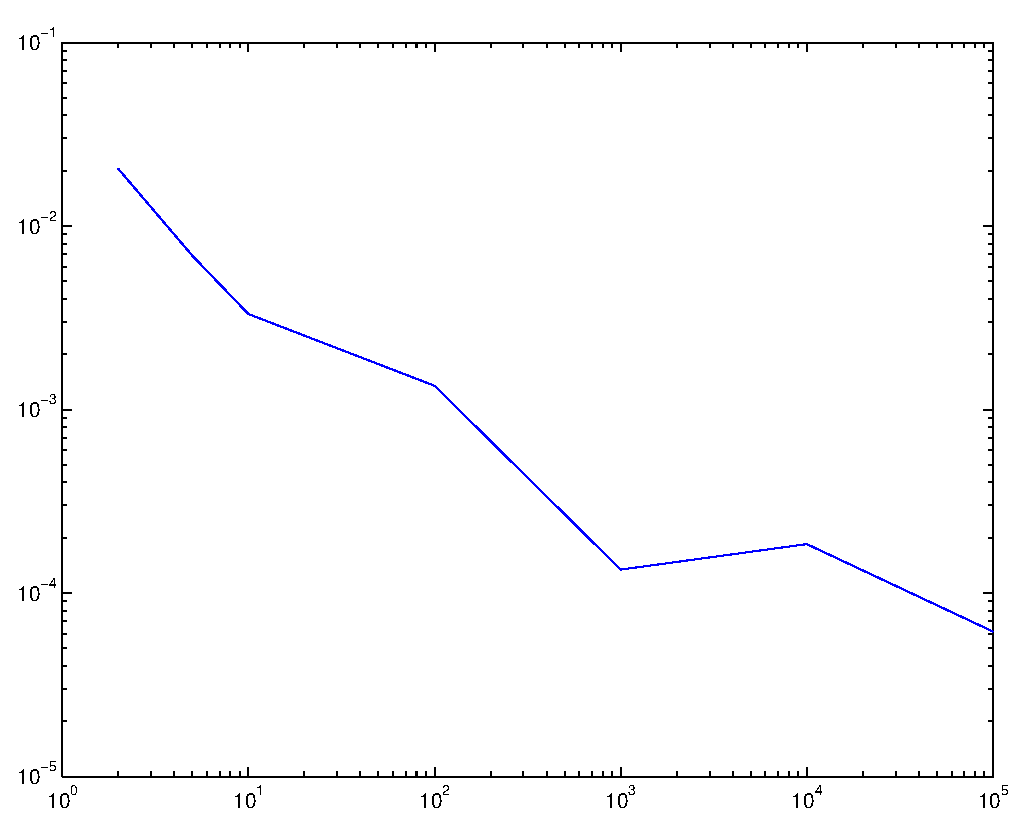
\includegraphics [scale=0.8] {log_plot.eps}




\end{enumerate}


% -----------end document --------------------
\end{document}